\ection{Test Application}\label{ssec:testApplication}
	In order to perform the test a \textit{LabView} application was developed to control the lower level hardware and perform data processing, the application main screen can be seen in Figure \ref{fig:labview-app-mainscreen}.

	\begin{figure}[htbp]
		\centering
		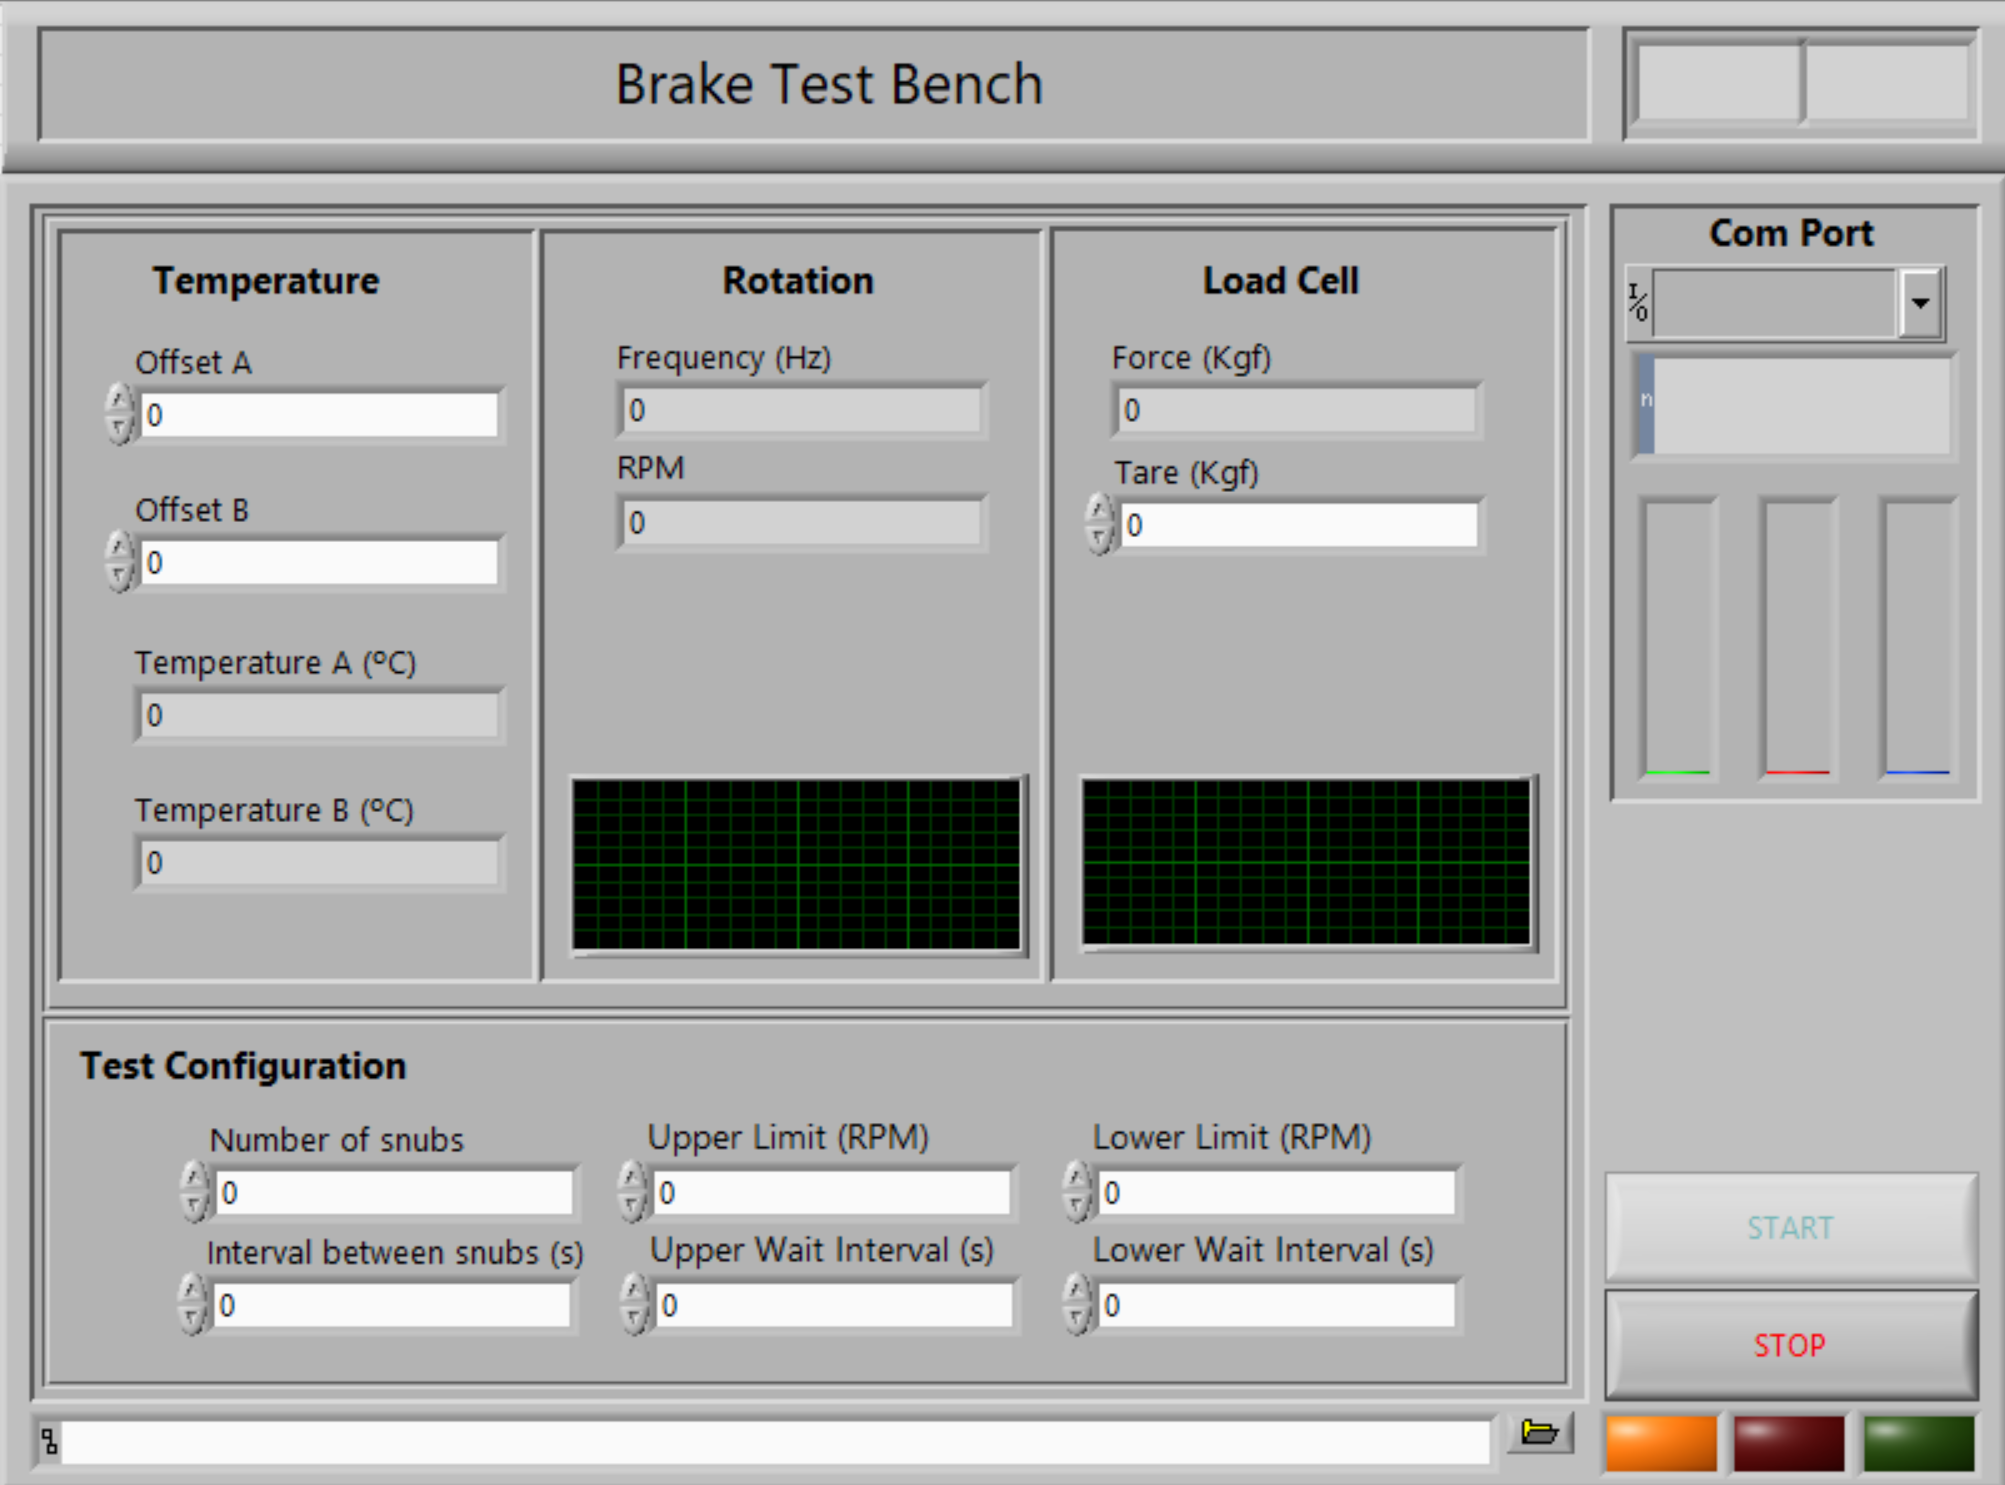
\includegraphics[scale=0.7]{figuras/fig-labview-app-mainscreen}
		\caption{Test Application Main Screen}
		\label{fig:labview-app-mainscreen}
	\end{figure}

	The main screen is divided in three parts, first part displays the sensors readings, thermocouples measured temperature, rotation frequency and RPMs and load cell braking force. On the bottom of the screen the test configurations, them being:

	\begin{itemize}Number of Snubs: 
		\item\textit{Number of Snubs:} The number of times each brake iteraction will be done.
		\item\textit{Interval between snubs (s):} The amount of seconds that a interface will wait at the end of a brake iteraction before accelerating the motor again.
		\item\textit{Upper Limit (RPM):} At each snub the system will accelerate the electric engine until the rotor reaches this pre-defined rotation rhythm.
		\item\textit{Upper Wait Interval (s):} After reaching the upper rotation limit the system will wait for this interval before braking.
		\item\textit{Lower Limit (RPM):} The system will perform braking until the rotor reaches this lower RPM limit.
		\item\textit{Lower Wait Interval (s):} After reaching the Lower Limit the system will for this interval.
	\end{itemize}

	The software itself will take full control of the test, it will turn the electric motor on when needed, turn the brakes one